\documentclass{article}

\usepackage{url}

\usepackage{amssymb,amsfonts,amsmath,amsthm,mathtools}
\usepackage{adjustbox}
\usepackage{float}
\usepackage{caption}
\usepackage{mdframed}
\usepackage{lmodern}
\usepackage{bm,bbold}
\usepackage{xfrac, nicefrac}
\usepackage{xcolor}
\usepackage{lmodern}
\usepackage{enumitem}
\usepackage{pgfplots, pgf,tikz}
\usepackage[margin=60pt]{geometry}
\pdfinclusioncopyfonts=1

\definecolor{RED}{HTML}{EB6231}
\definecolor{YELLOW}{HTML}{E29D26}
\definecolor{BLUE}{HTML}{5D80B4}
\definecolor{LIGHTGREEN}{HTML}{6ABD9B}
\definecolor{GREEN}{HTML}{8FB03E}
\definecolor{PURPLE}{HTML}{BE1E2D}
\definecolor{BROWN}{HTML}{A97C50}
\definecolor{PINK}{HTML}{DA1C5C}
\pgfplotsset{every axis/.append style={line width=1pt}}
\pgfplotscreateplotcyclelist{colors}{LIGHTGREEN\\YELLOW\\RED\\GREEN\\BLUE\\}
\captionsetup{width=0.85\textwidth}

\newcommand{\specialcell}[2][c]{%
	\begin{tabular}[#1]{@{}c@{}}#2\end{tabular}}

\DeclareMathOperator{\E}{\mathbb{E}}
\newcommand{\der}{\mathrm{d}}
\newcommand{\e}{\mathrm{e}}
\newcommand{\indice}{l}
\newcommand{\indiceexp}{^{(\indice)}}
\newcommand{\angstrom}{\text{\normalfont\AA}}

% Time, effective population size and mutation rate.
\newcommand{\Ne}{N_{\mathrm{e}}}
\newcommand{\dnds}{\omega}
\newcommand{\Nsite}{\text{n}}
\newcommand{\site}{\text{i}}
% DNA

\newcommand{\ci}{\mathbb{S}_{t}}
\newcommand{\cj}{\mathbb{S}_{t}'}
\newcommand{\itoj}{\ci, \cj}
\newcommand{\setNeighbors}{\mathcal{M}\left(\ci\right)}
\newcommand{\setNonSynNeighbors}{\mathcal{N}\left(\ci\right)}
\newcommand{\setSynNeighbors}{\mathcal{S}\left(\ci\right)}
\newcommand{\submatrix}{q}

\newcommand{\phenoDiv}{S}
\newcommand{\s}{s}
\newcommand{\pheno}{x}
\newcommand{\dpheno}{\delta \pheno}
\newcommand{\phenoFold}{\Delta G}
\newcommand{\phenoFoldMin}{\alpha}
\newcommand{\dphenoFold}{\gamma}

\begin{document}

\title{Substitution rate responses to changes in effective population size.}

\author{T. Latrille, N. Lartillot}
 
\maketitle
 
\abstract{
The substitution rate of selected mutations relative to the substitution rate of neutral mutation ($\dnds$) had been theoretically expected to decrease with effective population size ($\Ne$).
Mechanistically, populations with high $\Ne$ would have stronger purifying selection, hence lower $\dnds$, due to the decrease of random drift.
Such theoretical prediction had been observed in empirical data across many clades.
However, several studies failed to observe such response of $\dnds$ to changes in $\Ne$, or with weak strength or direction.
Computational model of protein folding have shown that $\dnds$ can be independent of $\Ne$, which can mathematical be proven under certain assumptions.
Moreover, non-equilibrium properties can implies that an increase of $\Ne$ can result first in an increase of $\dnds$ and then a decrease.
Together, assumptions about the mapping of sequence to fitness can display a variety of behaviours in the $\dnds$ responses to changes in $\Ne$.
Our goal in this present work to reconcile empirical observation with theoretical results, such as to delimit which models and assumptions are reasonable.
We provide a simple mechanistic model that can display a wide range of behaviours depending on the parametrization.
Our result show that models assuming site-specific fitness landscapes (without epistasis) is at risk of over-estimating the time taken to reach the new equilibrium value of $\dnds$ after a change in $\Ne$, but paradoxically also over-estimating the equilibrium $\dnds$ response to changes in $\Ne$.
}

\section{Introduction}
Differences in DNA sequences of a gene in separate species are due to the particular history of DNA substitutions along each specie's respective lineage.
These substitutions  at the level of the population are the result of point mutations at the level of individuals, subject to evolutionary forces such as selection and random drift.
In protein-coding DNA sequences, non-synonymous mutations are changing the amino-acid sequence, and by comparing the non-synonymous substitutions rate relative to the synonymous substitution rate (supposedly neutral), a statistic called $\dnds$, we can estimate the global strength of selection and random drift.\\

For a given gene, it has been empirically observed changes of $\dnds$ along lineages of a phylogeny \cite{Yang2001, Zhang2004}.
More importantly, changes in substitution rate correlate with changes in life-history-traits (longevity, body mass, ...) such as shown by the molecular comparative framework \cite{Lartillot2011,Weber2014}.
Such covariation are compatible with the theoretical prediction of the nearly-neutral theory of evolution \cite{Ohta1972, Ohta1992}, where the underlying mechanism is changes in effective population size ($\Ne$).
Indeed, populations with low $\Ne$ would have both a large body size and a high $\dnds$ (weaker selection) due to the increase of random drift.
If $\dnds$ is empirically correlated to life-history traits, such as body mass and longevity, the direction of correlation could not be replicated across all experiments \cite{Figuet2016}.\\

Theoretical prediction of $\dnds$ decreasing as a function of $\Ne$ had been developed in the context of a fixed distribution of fitness effects \cite{Ohta1972, Welch2008}, and also been shown in context of a fixed fitness landscape, where each amino-acid have different fitnesses \cite{Spielman2015a, DosReis2015}.
However, it has also been argued that the existence of a $\dnds$ response to $\Ne$ is not straightforward, even in the context of nearly-neutral theory of evolution \cite{Lanfear2014}.
In the example of a bio-chemical mechanistic computational model, where the fitness is determined by the probability of folding, $\dnds$ is independent of $\Ne$ \cite{Goldstein2013}.
Theoretically, a more general case is obtained whenever the fitness is a concave function of a trait, and such trait is equimutable \cite{Cherry1998}.
Equimutabibilty meaning a mutation has the same effect on the trait whatever the current trait of the individual.
Moreover, even in the case of a $\dnds$ response to $\Ne$, this response is far from being $1$-to-$1$ due to non-equilibrium properties, such that an increase in $\Ne$ implies firstly a burst of $\dnds$, and subsequentially a decrease in $\dnds$ \cite{Jones2016}.\\

Our goal in this present work to reconcile empirical observation with theoretical results, such as to delimit which models and assumptions are reasonable.
This question is important if we want to extract changes in effective population size from substitution history, as well as to determine the fitness landscape under which protein-coding DNA sequences are evolving.

\section{Results}
\subsection{$\bm{\dnds}$ at equilibrium as a function of $\bm{\Ne}$}

We provide a simple toy model, with $2$ parameters that shows a variety of behaviours. 
This model map the amino-acid sequence to the free energy (kcal/mol) between folded and unfolded state of the whole protein.
Each amino-acid site in the protein can be in the unstable or stable state.
A protein is optimal ($\phenoFold = \phenoFoldMin$) if all amino-acids are in the stable state.
Each amino-acid destabilizing the protein brings an increase of $\phenoFold$ equal to $\dphenoFold$.
\begin{equation}
\phenoFold = \phenoFoldMin + \dphenoFold * d, 
\end{equation}
where $d$ is the number of unstable amino-acid sites in the sequence, $\alpha$ and $\gamma$ are in kcal/mol.
Wrightian fitness is defined as the probability of our protein to be in the folded state, given by Boltzmann equation: 
\begin{equation}
w(\phenoFold) = \dfrac{1}{1 + e^{\beta \phenoFold }}, 
\end{equation}
where $\beta=1.686$ mol/kcal at room temperature.\\

In the original studies \cite{Williams2006, Goldstein2011, Pollock2012}, free energy of the folded state is computed using the $3$D structure of the folded state and pair-wise contact energies between neighboring amino-acid residues using Miya-zawa \& Jernigan contact potentials \cite{Miyazawa1985}.
The free energy distribution of unfolded states is approximated using $55$ decoy $3$D structures that supposedly represent a sample of possible unfolded states (see Supplementary Materials).\\

The parameters $\alpha$ and $\gamma$ of our toy model are set to match the average values observed in the original model.
$\alpha=-118$ kcal/mol, as it is the $\phenoFold$ of the most stable sequence of $300$ sites \cite{Goldstein2011}.
$\gamma=1.0$ kcal/mol, as the average observed increase in $\phenoFold$ per destabilizing mutation \cite{Zeldovich2007}.

\begin{figure*}[htb!]
\begin{mdframed}
	\centering
	\includegraphics[width=\textwidth] {artworks/XPopSizeYOmegaEq.pdf}
	\vspace*{0.2em}
	\caption{
		\textbf{$\bm{\dnds}$ response to change in $\bm{\Ne}$}.
		Panel A. Our toy model reproduces the observations of Goldstein \cite{Goldstein2013} that $\dnds$ at equilibrium is independent of $\Ne$. Indeed, whenever the parameters $\alpha$ and $\gamma$ are taken to match the average values observed in the original model, we observed no response of $\dnds$ to $\Ne$ (pink and brown lines).
		However, decreasing both $\alpha$ and $\gamma$ together implies a strong negative relationship between $\Ne$ and $\dnds$, as predicted under the nearly-neutral theory of evolution.
		Panel B. By reducing the number of sites of the protein, thus by effectively reducing the potential number of sites that can compensate for the change in $\Ne$, the $\dnds$ response to changes in $\Ne$ is stronger.
	}
	\label{fig:EqdndsNe}
\end{mdframed}
\end{figure*}

DNA sequence evolution are simulated under an origin-fixation model \cite{McCandlish2014}, where the rate of substitution of a new mutation with selection coefficient $s$ is:
\begin{equation}
p_{\text{fix}}(s) = \mu \dfrac{4 \Ne s}{1 + e^{- 4 \Ne s }}, 
\end{equation}
where $\mu$ is the mutation rate.\\

Our toy model reproduces the observations that $\dnds$ at equilibrium is independent of $\Ne$. Indeed, whenever the parameters $\alpha$ and $\gamma$ are taken to match the average values observed in the original model, we observed no response of $\dnds$ to $\Ne$.
However, decreasing both $\alpha$ and $\gamma$ together implies a strong negative relationship between $\Ne$ and $\dnds$, as predicted under the nearly-neutral theory of evolution.
Moreover, by reducing the number of sites of the protein, thus by effectively reducing the potential number of sites that can compensate for the change in $\Ne$, the $\dnds$ at equilibrium after changes in $\Ne$ is stronger \textit{Necessary mechanistic explanation for this fact} (see Figure \ref{fig:EqdndsNe}).

\subsection{Epistasis determines the time to relaxation}

Although the equilibrium value of $\dnds$ after changes in $\Ne$ is an important feature of the $\dnds$-$\Ne$ relationship, an other parameter that is often neglected is the relaxation time to reach the new equilibrium $\dnds$ \cite{Jones2016}.
\begin{figure*}[htb!]
\begin{mdframed}
	\centering
	\includegraphics[width=\textwidth]{artworks/SimuStabExponentialDecay.png}
	\vspace*{0.2em}
	\caption{
		\textbf{$\bm{\dnds}$ relaxation time to changes in $\bm{\Ne}$}.
		Panel A. Our result show that with low epistasis, the time taken to reach the new equilibrium value of $\dnds$ after a change in $\Ne$ is long, such that relaxation rate is on the order of the mutation rate.
		Panel B. With high epistasis, the relaxation time is short.
	}
	\label{fig:relaxStability}
\end{mdframed}
\end{figure*}
In the case of a fitness landscape with epistasis, after a change in $\Ne$, any site that is used to climb either up or down the fitness landscape will have diminishing return in other site of the sequences.
Not taking into account epistasis have the consequence of over-estimating the relaxation time to return to equilibrium of $\dnds$ after changes in $\Ne$ \ref{fig:relaxStability}).

Using a site-specific fitness landscape, where each amino-acid have different fitnesses, thus with no epistasis, the relaxation time is long since every site has to adapt to the new change in $\Ne$.
However, using a distribution of fitness effect (DFE) does not suffer from under-estimating the relaxation rate, since the effect is instantaneous (see Figure \ref{fig:relaxProfileDFE}).

\begin{figure*}[htb!]
\begin{mdframed}
	\centering
	\includegraphics[width=\textwidth]{artworks/SimuExponentialDecay.png}
	\vspace*{0.2em}
	\caption{
		\textbf{$\bm{\dnds}$ relaxation time under different fitness models.}.
		Panel A. In context of a fixed fitness landscape, where each amino-acid have different fitnesses (site-specific profile), the time taken to reach the new equilibrium value of $\dnds$ after a change in $\Ne$ is long, such that relaxation rate is on the order of the mutation rate.
		Panel B. In the context of a distribution of fitness effects, the relaxation time is non-existent.
	}
	\label{fig:relaxProfileDFE}
\end{mdframed}
\end{figure*}

\section{Discussion}

Goldstein \& Pollock argued that model of protein evolution should consider how the acceptance of mutations depends on the sequence context in which they arise (epistasis), as to correctly represent resultant rate heterogeneity along the sequence, to predict the role of compensatory substitutions in protein evolution, predict which of the 10\% of deleterious mutations in humans are harmless in other species, or to accurately represent the rate and time dependence of convergence and homoplasy \cite{Goldstein2017}.
We argue that not taking into account epistasis also have the consequence of over-estimating the relaxation time to return to equilibrium of $\dnds$ after changes in $\Ne$.
Paradoxically, not taking into account epistasis means over-estimating the response of $\dnds$ to changes in $\Ne$ at equilibrium.\\

If using a distribution of fitness effect (DFE) is mathematically convenient and does not suffer from under-estimating the relaxation rate, it is also over-estimating the response of $\dnds$ to changes in $\Ne$ at equilibrium (\textit{should show proof and mechanistic explanation that the selection coefficient shall not be independent of $\Ne$}).
As such, developing inference of fitness landscape will require to assume site-interdependent fitness landscapes.\\

Our model does not display site variation in $\dnds$, which is a strong limitation, as it has observed in most protein \cite{Echave2017}.
\section{Materials \& Methods}

\subsection{Simulation with protein folding probability}
\label{MatMet:folding}
From a DNA sequence $\ci$ after $t$ substitutions, the protein's difference in free energy between folded and unfolded state is given by:
\begin{equation*}
\phenoFold\left(\ci\right) = \phenoFoldMin + \dphenoFold * d\left(\ci\right), 
\end{equation*}
where $d\left(\ci\right)$ is the number of non-optimal amino-acid sites in the sequence.
Wrightian fitness is defined as the probability of our protein to be in the folded state, given by the Boltzmann equation: 
\begin{equation}
w(\phenoFold\left(\ci\right)) = \dfrac{P_{\mathrm{F}}\left(\ci\right)}{P_{\mathrm{F}}\left(\ci\right) + P_{\mathrm{U}}\left(\ci\right)} = \dfrac{e^{-\beta G_{\mathrm{F}}\left(\ci\right) }}{e^{-\beta G_{\mathrm{F}} \left(\ci\right) } + e^{-\beta G_{\mathrm{U}}\left(\ci\right) }} = \dfrac{1}{1 + e^{\beta \phenoFold\left(\ci\right) }}, 
\end{equation}
where $\beta$ is the inverse of the temperature ($\beta=1/kT$).

From the resident sequence $\ci$, we define $\setNeighbors$ as the set of all possible mutant that are one nucleotide away from $\ci$, and were mutant sequences containing a stop codon are excluded.
For a protein of $\Nsite$ amino-acid sites, $\left| \setNeighbors \right| \leq 9 \Nsite$, since each codon has a maximum of $9$ possible mutant codon that are one mutation away and that are not stop codon.
For each mutant sequence $\cj \in \setNeighbors$, we compute $\phenoFold^{t+1}$ from the updated sequence $\cj$, and subsequently the selection coefficient of the mutant:
\begin{equation}
s \left( \ci,\cj\right) = \dfrac{ w\left( \phenoFold\left(\cj\right) \right) - w\left( \phenoFold\left(\ci\right) \right)}{w\left( \phenoFold\left(\ci\right) \right)}.
\end{equation}
The next change in the protein coding DNA and the time to next the event is chosen using Gillespie algorithm, according to the rates of substitution between codons:
\begin{equation}
\submatrix_{\itoj} = \mu_{\itoj} \dfrac{4 \Ne s \left( \ci,\cj\right)}{1 - \e^{-4 \Ne s \left( \ci,\cj\right)}}, 
\end{equation}
where $\mu_{\itoj}$ is the mutation rate between $\ci$ and $\cj$, determined by the underlying $4x4$ nucleotide mutation rate matrix, and ${\submatrix_{\itoj}} = \mu_{\itoj}$ in the case of synonymous substitutions.


\subsection{Simulation with independent fitness profiles}
A fitness profile give a fitness for each amino-acid (vector of size $20$).
Each site of the protein has a specific amino-acid fitness profile.
Overall, the protein phenotype is computed as the sum of site-specific selection coefficient, obtained by accessing the amino-acid present at each site of the protein.
The selection coefficient of the mutant $\cj$ is:
\begin{equation}
s \left( \ci,\cj\right) = \sum_{1 \leq \site \leq \Nsite} \ln \left( \dfrac{G_{\site} \left(\cj(\site) \right)}{G_{\site} \left(\ci(\site) \right)} \right) ,
\end{equation}
where $G_{\site}$ is the fitness profile at site $\site$, obtained in empirical experiment \cite{Bloom2017}.
\begin{center}
	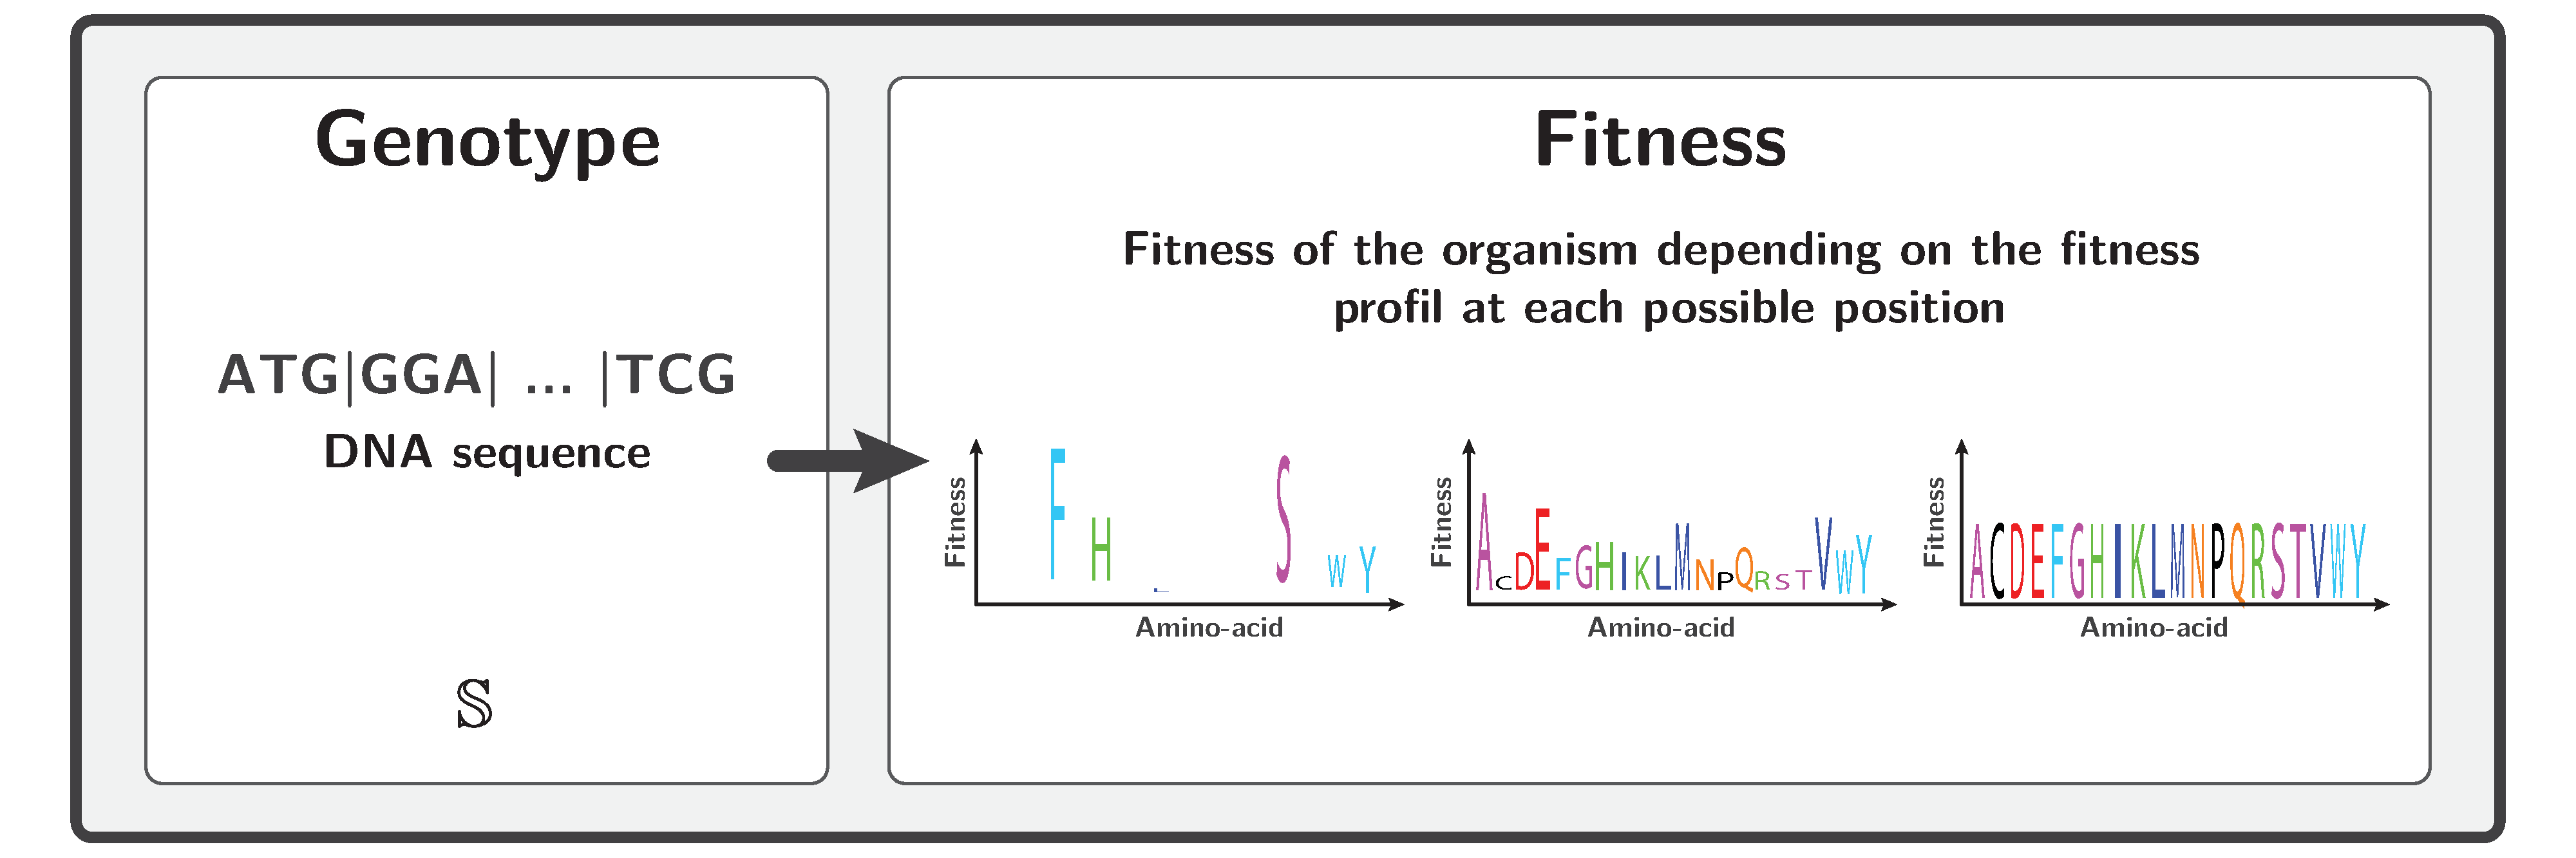
\includegraphics[width=165mm] {artworks/ModelSimuDiv.pdf}
\end{center}

The next change in the protein coding DNA and the time to next the event is chosen using Gillespie algorithm, as in \ref{MatMet:folding}.

\subsection{Simulation with distribution of fitness effects}
The selection coefficient of the mutant $\cj$ is gamma distributed (shape $\beta > 0$):
\begin{equation}
- s \left( \ci,\cj\right) \sim \text{Gamma} \left( \bar{|s|}, \beta \right)
\end{equation}
The next change in the protein coding DNA and the time to next the event is chosen using Gillespie algorithm, as in \ref{MatMet:folding}.

\subsection{$\bm{\dnds}$ along the simulation}
From the set of mutant $\setNeighbors$ that are one nucleotide away from $\ci$, we define the subsets $\setNonSynNeighbors$ and $\setSynNeighbors$ that are respectively the set of non-synonymous and synonymoys mutants, where  $\setNonSynNeighbors \cup \setSynNeighbors = \setNeighbors$.
As in previous works \cite{Spielman2015a, DosReis2015, Jones2016}, the ratio of non-synonymous over synonymous substitution rates of the sequence is defined as :
\begin{align}
\dnds(t) &= \dfrac{\sum_{\cj \in \setNonSynNeighbors} \submatrix_{\itoj}}{\sum_{\cj \in \setNonSynNeighbors} \mu_{\itoj}} \left( \dfrac{\sum_{\cj \in \setSynNeighbors} \submatrix_{\itoj}}{\sum_{\cj \in \setSynNeighbors} \mu_{\itoj}} \right)^{-1}\\
 &= \dfrac{\sum_{\cj \in \setNonSynNeighbors} \mu_{\itoj} \dfrac{4 \Ne s \left( \ci,\cj\right)}{{1 - \e^{-4 \Ne \left( \ci,\cj\right)} }}}{\sum_{\cj \in \setNonSynNeighbors} \mu_{\itoj}} 
\end{align}
\subsection{Reproducibility}
The simulators written in C++ are publicly available under MIT license at \url{https://github.com/ThibaultLatrille/SimuEvol}.
The scripts and instructions necessary to reproduce the experiments are available at \url{https://github.com/ThibaultLatrille/GenotypePhenotypeFitness}.

\bibliographystyle{apalike}
\bibliography{refs-codons,refs-cds}

\newpage
\part*{Supplementary materials}

\section*{Probability of folding as in Goldstein \& Pollock}
We simulated substitutions in the protein phosphatase ($\Nsite=300$ codon sites).
From a DNA sequence $\ci$ after $t$ substitutions, we compute the free energy of the folded state $G_{\mathrm{F}}\left(\ci\right)$, using the $3$-dimensional structure of the folded state and pair-wise contact energies between neighboring amino-acid residues:
\begin{equation}
G_{\mathrm{F}}\left(\ci\right) = \sum_{1 \leq \site \leq \Nsite} \sum_{r \in \mathcal{N}(\site)} I \left(\ci(\site), \ci(r) \right),
\end{equation}
where $I(a,b)$ is the pair-wise contact energies between amino-acid $a$ and $b$, using contact potentials estimated by Miya-zawa and Jernigan, and $\mathcal{N}(\site)$ are the neighbor residues of site $\site$ (closer than $7\angstrom$) in the $3$D structure.\\

The free energy of unfolded states $G_{\mathrm{U}}\left(\ci\right)$ is approximated using $55$ decoy $3$D structures that supposedly represent a sample of possible unfolded states:
\begin{equation}
G_{\mathrm{U}}\left(\ci\right) = \langle G\left(\ci\right) \rangle - kT \ln (1.0\mathrm{E}^{160}) - \dfrac{2 \left[ \langle G\left(\ci\right)^2 \rangle - \langle G\left(\ci\right) \rangle^2\right] }{kT}
\end{equation}
where the average $\langle . \rangle$ runs other the $55$ decoy $3$D structures, and $k$ is the Boltzmann constant and $T$ the temperature in Kelvin.\\

From the energy of folded and unfolded states, we can compute the difference in free energy between the states:
\begin{equation}
\phenoFold\left(\ci\right) = G_{\mathrm{F}}\left(\ci\right) - G_{\mathrm{U}}\left(\ci\right)
\end{equation}

\begin{center}
	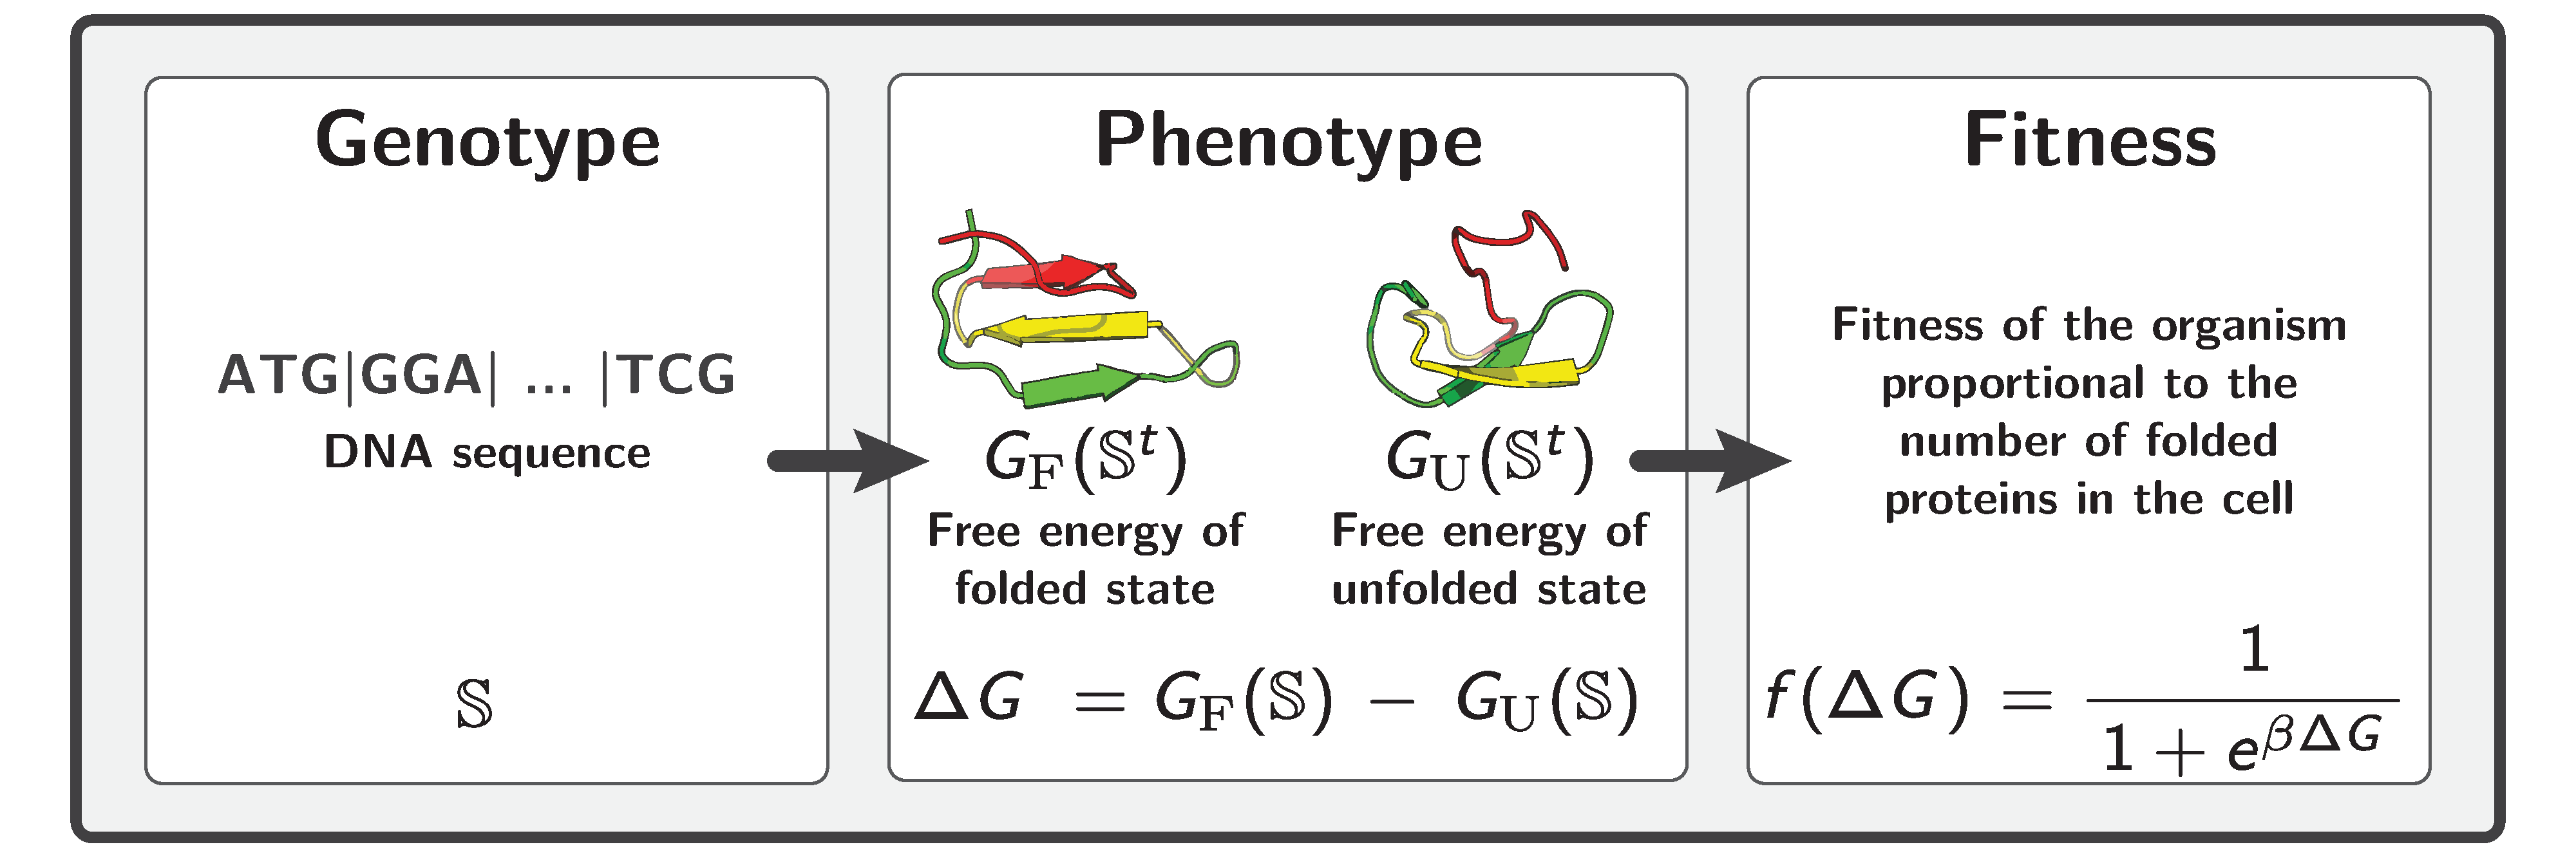
\includegraphics[width=165mm] {artworks/ModelSimuFold.pdf}
\end{center}

\section*{Equimutability}
We define $\pheno$ as the current phenotype and $\dpheno$ as the phenotypic effect of a mutation.
$\s \left( \pheno, \dpheno \right)$ is the selection coefficient of a phenotypic effect $\dpheno$ if the current phenotype is $\pheno$:
\begin{equation*}
\s \left( \pheno, \dpheno \right) = \dfrac{w \left( \pheno + \dpheno \right) - w \left( \pheno \right)}{w \left( \pheno \right)} \simeq w'\left( \pheno \right) \dpheno, 
\end{equation*}
where $w \left( \pheno \right)$ is the Wrightian fitness of phenotype $x$.
We also define $\rho_{\pheno}(\dpheno)$ as the distribution of phenotypic effects, at phenotype $\pheno$.
At equilibrium, the expected selection coefficient $ 4 \Ne \s \left( \pheno, \dpheno \right)$ of mutations that reached fixation must be $0$:
\begin{align*}
0 & = \E_{\dpheno} \left[ 4 \Ne \s\left( \pheno, \dpheno \right) \dfrac{ 4 \Ne \s\left( \pheno, \dpheno \right) }{1 - \e^{4\Ne\s\left( \pheno, \dpheno \right)}} \right] \\ & 
\simeq \int_{-\infty}^{\infty} \dfrac{ \left[ 4 \Ne f'\left( \pheno \right)  \right]^2}{1 - \e^{4\Ne f'\left( \pheno \right) \dpheno} }  \dpheno^2  \rho_{\pheno}(\dpheno) \der \dpheno 
\end{align*}
And the substitution rate is :
\begin{align*}
\omega(\Ne) & = \E_{\dpheno} \left[ \dfrac{ 4 \Ne \s \left( \pheno, \dpheno \right)}{1 - \e^{4\Ne \s \left( \pheno, \dpheno \right)}} \right] \simeq \E_{\dpheno} \left[ \dfrac{ 4 \Ne f'\left( \pheno \right) \dpheno}{1 - \e^{4\Ne f'\left( \pheno \right) \dpheno}} \right] \\
& \simeq \int_{-\infty}^{\infty} \dfrac{4 \Ne f'\left( \pheno \right) \dpheno}{1 - \e^{4\Ne f'\left( \pheno \right) \dpheno } } \rho_{\pheno}(\dpheno) \der \dpheno \\
\end{align*}
If $\rho_{\pheno}(\dpheno) = \rho(\dpheno)$ is independent of $\pheno$:
\begin{align*}
0 & \simeq \int_{-\infty}^{\infty} \dfrac{ \left[ 4 \Ne f'\left( \pheno \right)  \right]^2}{1 - \e^{4\Ne f'\left( \pheno \right) \dpheno} } \dpheno^2 \rho(\dpheno)  \der \dpheno \\
\Longrightarrow & \ 4 \Ne f'\left( \pheno \right) = K \in \mathbb{R}^{*} \text{ and } \s\left( \pheno, \dpheno \right) \simeq \dfrac{K \dpheno}{4\Ne} \\
\Longrightarrow & \ \omega( \Ne ) \simeq \int_{-\infty}^{\infty} \dfrac{ K  }{1 - \e^{K \dpheno } } \dpheno \rho(\dpheno)  \der \dpheno  \text{ is independent of } \Ne
\end{align*}


\end{document}